Zum Ende des Semesters treten alle Clients in einem gro"sen Turnier gegeneinander an, um die G\"ute der Clients festzustellen.
Zu diesem Turnier muss jedes Team vier Karten anfertigen, die speziell f\"ur ihren Client optimiert sind.
Dabei muss eine Zwei-, Drei-, Vier- und Achtspielerkarte eingereicht werden.
Bei den nachfolgend vorgestellten Karten handelt es sich jeweils um Maps, ann\"ahernd der Gr\"o"se 50x50.
Dies liegt daran, dass es sehr gute Algorithmen ben\"otigt um auf solchen Karten gute Z\"uge herauszusuchen.
Damit kann die G\"ute der einzelnen Clients besser \"uberpr\"uft werden.
Die Karten sind alle symmetrisch aufgebaut, wodurch eine gewisse Fairness gegeben ist.

\subsection{Comp2021 - Zweispielerkarte}\label{subsec:comp2021-2p}

\vspace{1em}
\begin{minipage}{\linewidth}
    \centering
    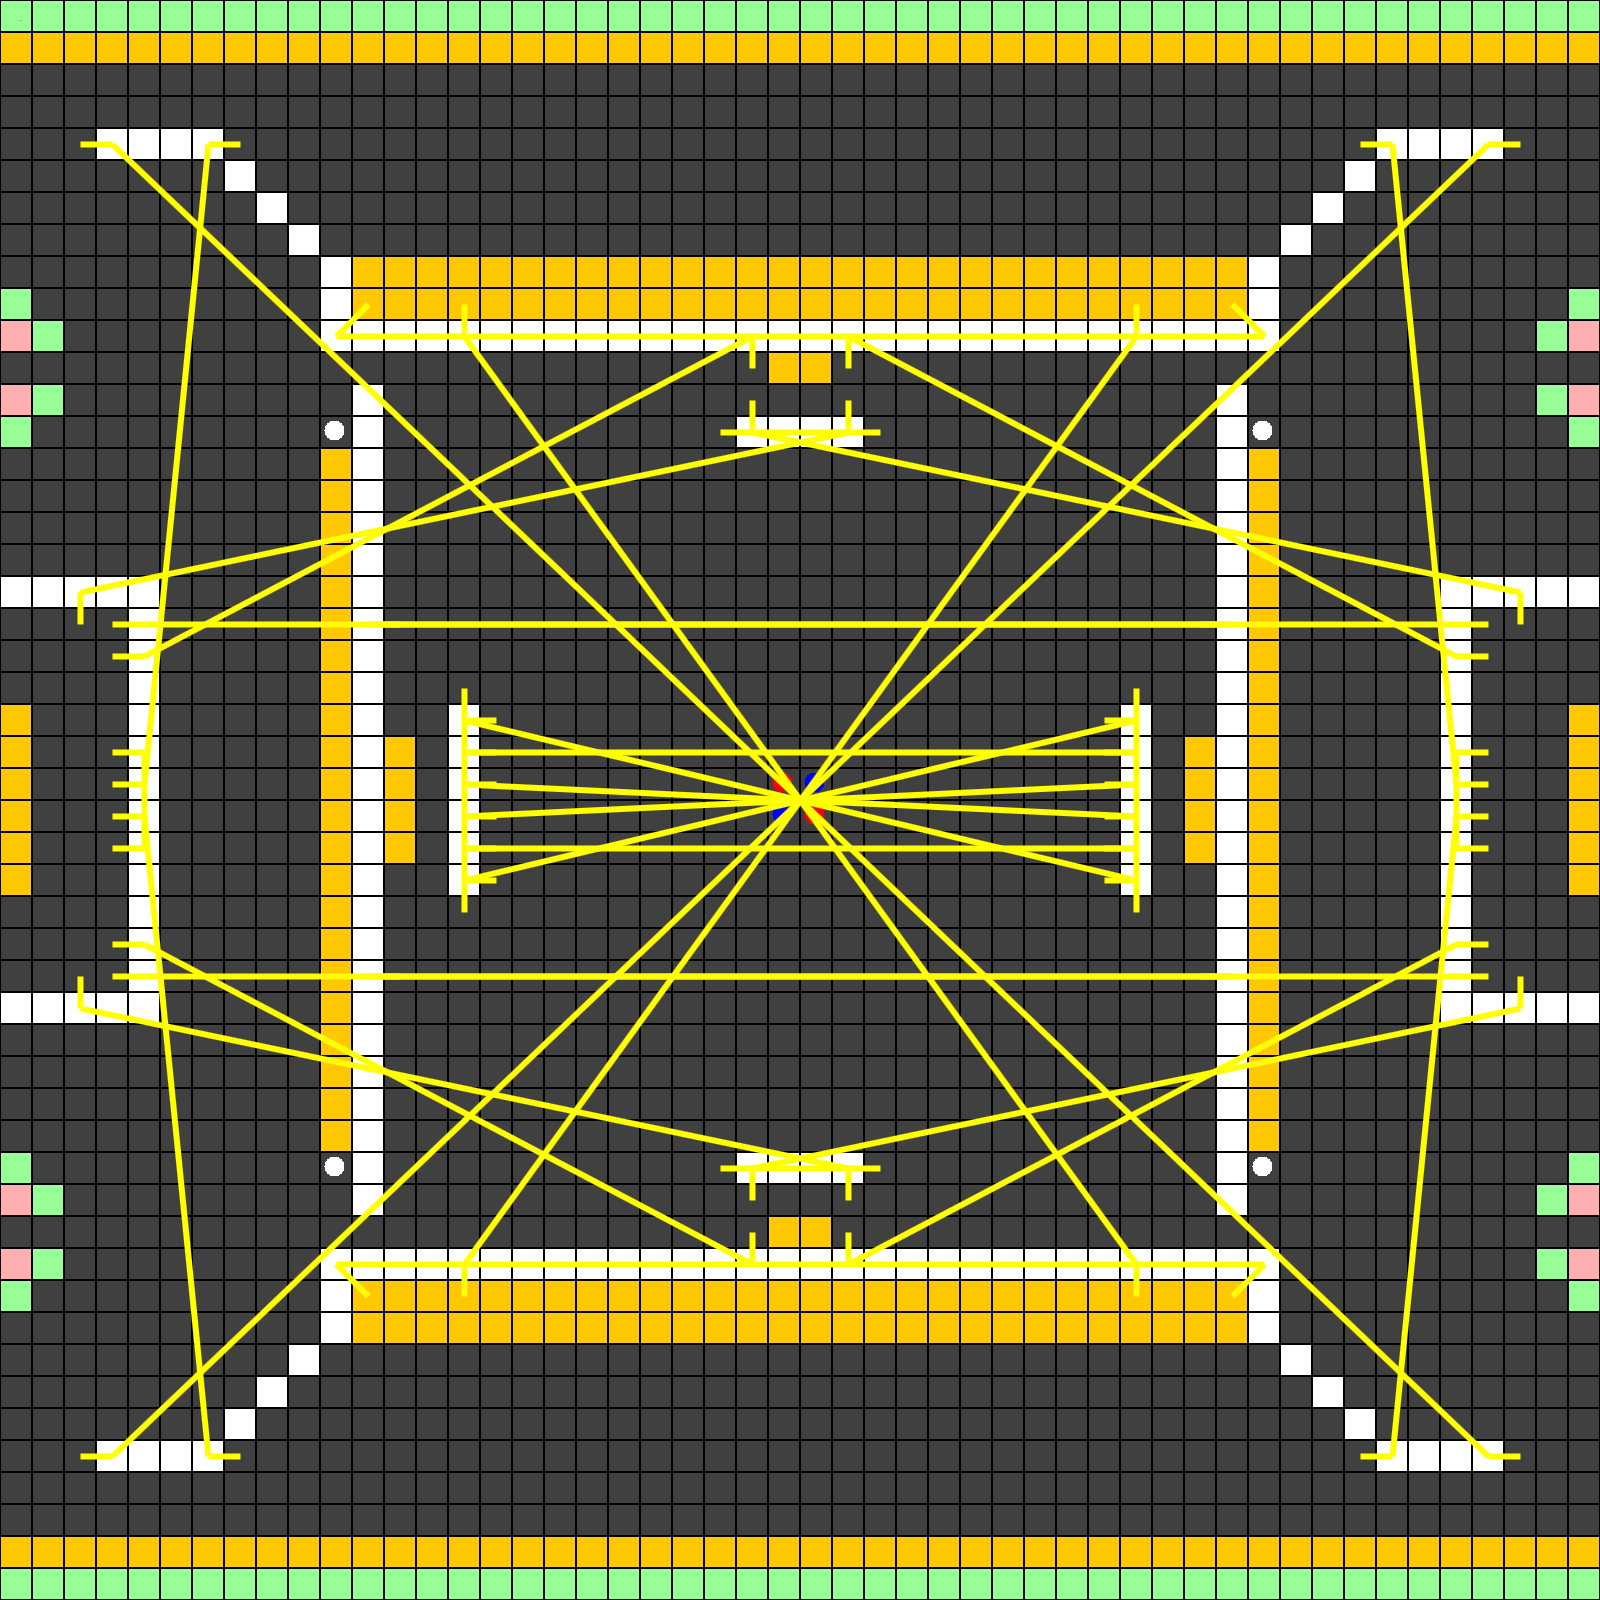
\includegraphics[width=0.49\linewidth]{pics/maps/comp2021_01_2p}
    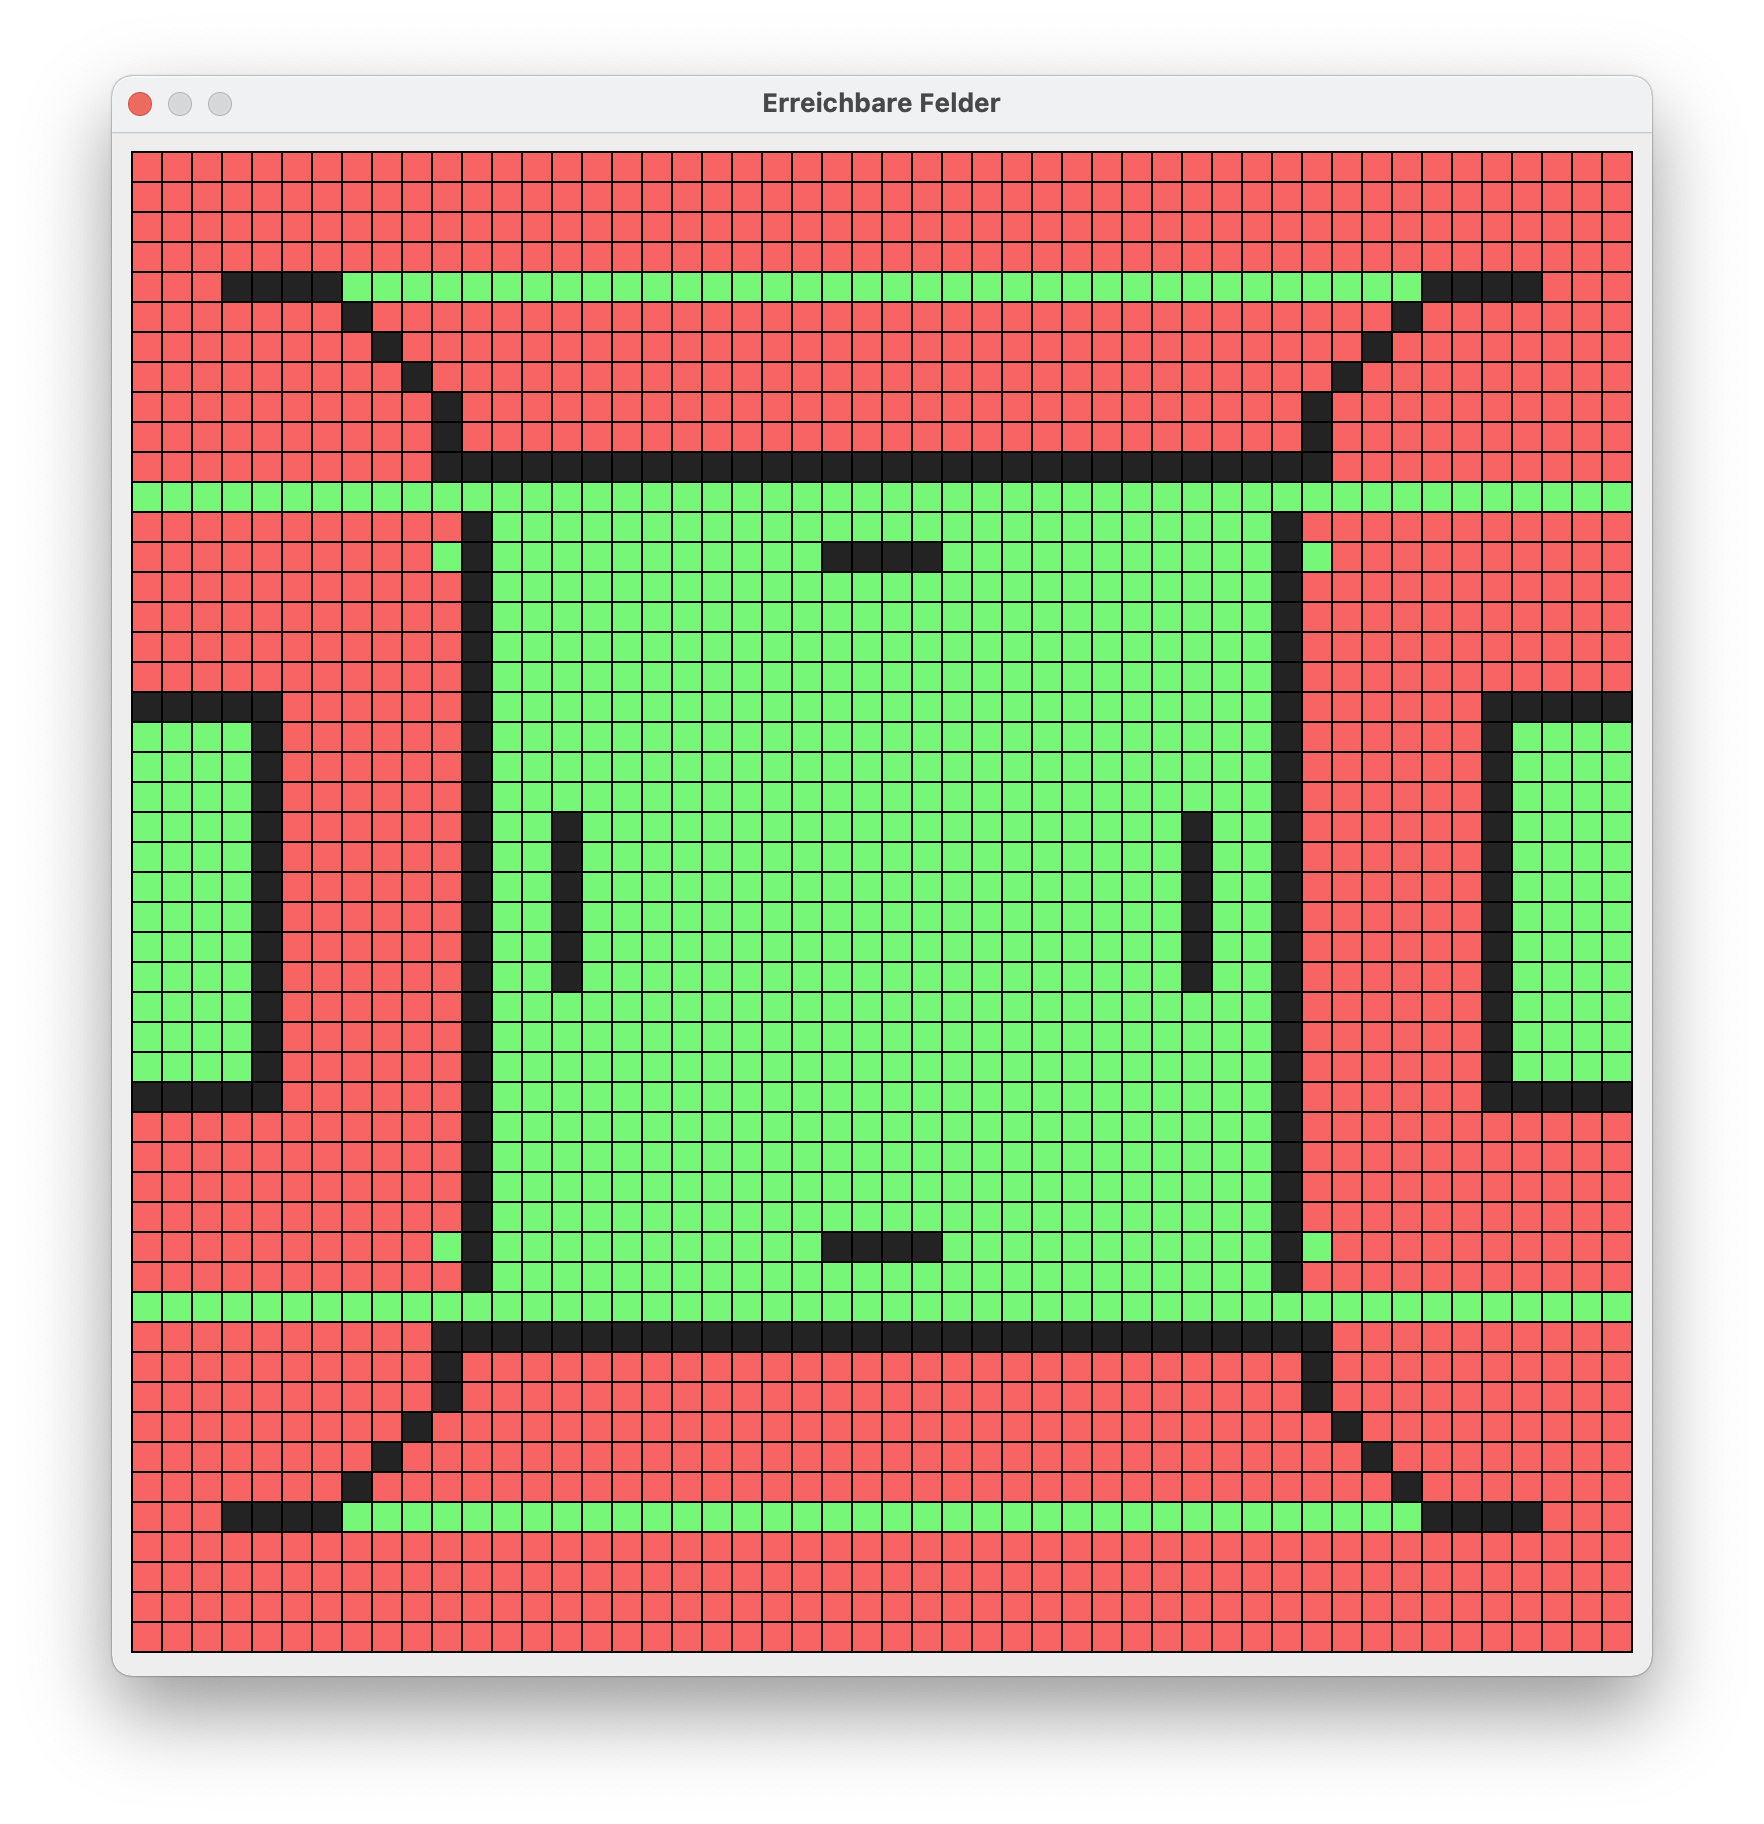
\includegraphics[width=0.48\linewidth]{pics/maps/field2021_01_2p}
    \captionof{figure}[Comp2p]{Zweispielerkarte inkl. erreichbare Felder in Gr\"un (rechts)}
    \label{fig:comp-2p}
\end{minipage}
\vspace{1em}

Bei dieser Karte handelt es sich um eine sehr gro"se Karte bezogen auf die Spielerzahl.
Genau hier wird jedoch auch der Vorteil des MapAnalyzers erkennbar.
Bei Karten, die sehr gro"se Teile nicht bespielbarer Felder haben, n\"utzt der MapAnalyzer extrem viel.
Es werden hier nicht nur Felder herausgerechnet, sondern auch Spezialsteine die nicht erreichbar sind f\"ur die sp\"atere Analyse unkenntlich gemacht.
Man erh\"alt somit eine adequatere Aussage \"uber den prozentualen Spielverlauf und eine realit\"atsnahere Vorstellung der Karte, wie diese bespielt werden kann.
Zudem gibt es Transitionen die nicht gezogen werden k\"onnen, da die dazu bn\"otigten Spielfelder nicht erreichbar sind.
Dieser Client kann mithilfe von Hashtabellen sehr effizient damit umgehen, wodurch keine Performanceeinbu"sen entstehen.

\subsection{Comp2021 - Dreispielerkarte}\label{subsec:comp2021-3p}

\vspace{1em}
\begin{minipage}{\linewidth}
    \centering
    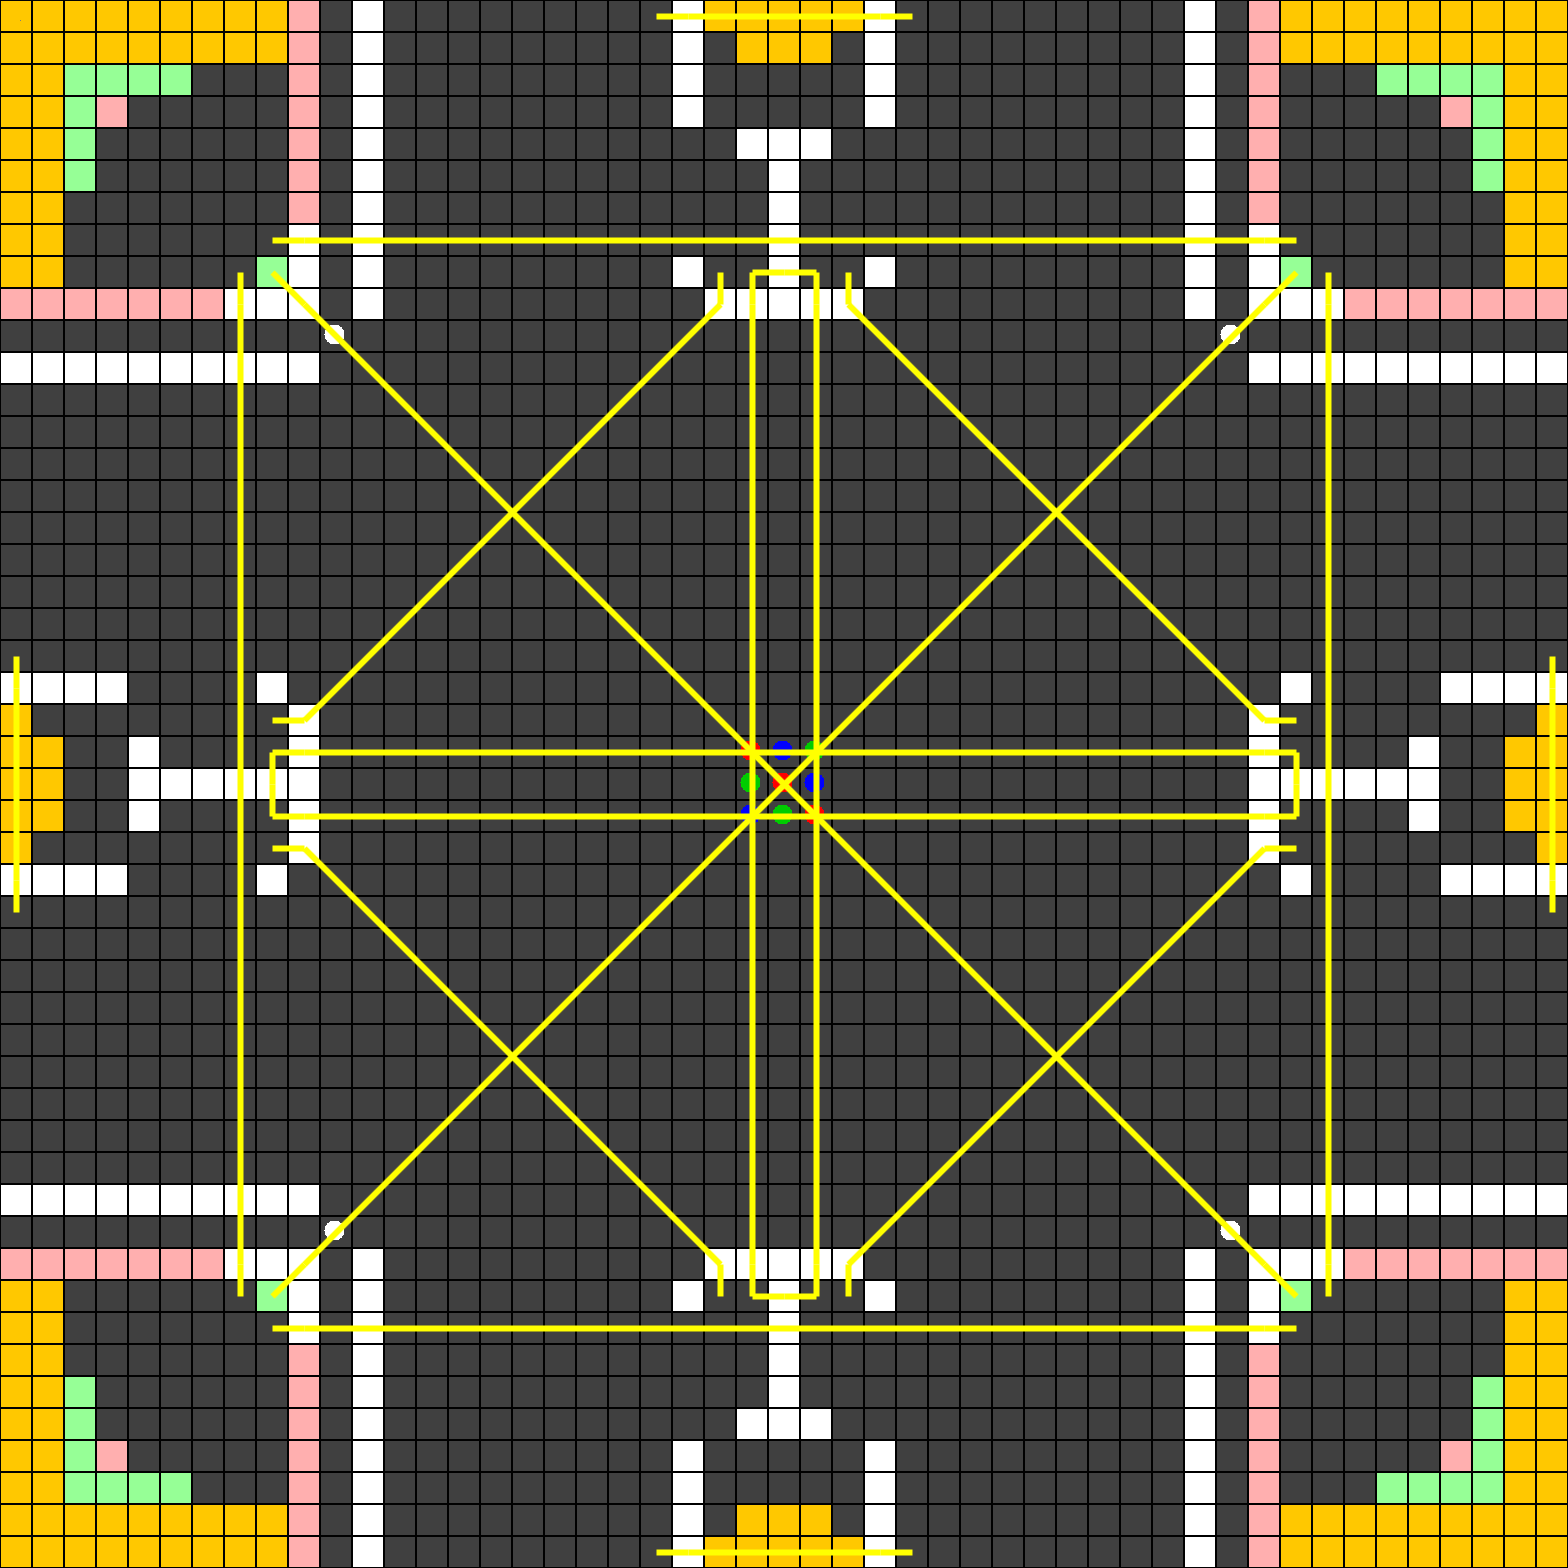
\includegraphics[width=0.49\linewidth]{pics/maps/comp2021_01_3p}
    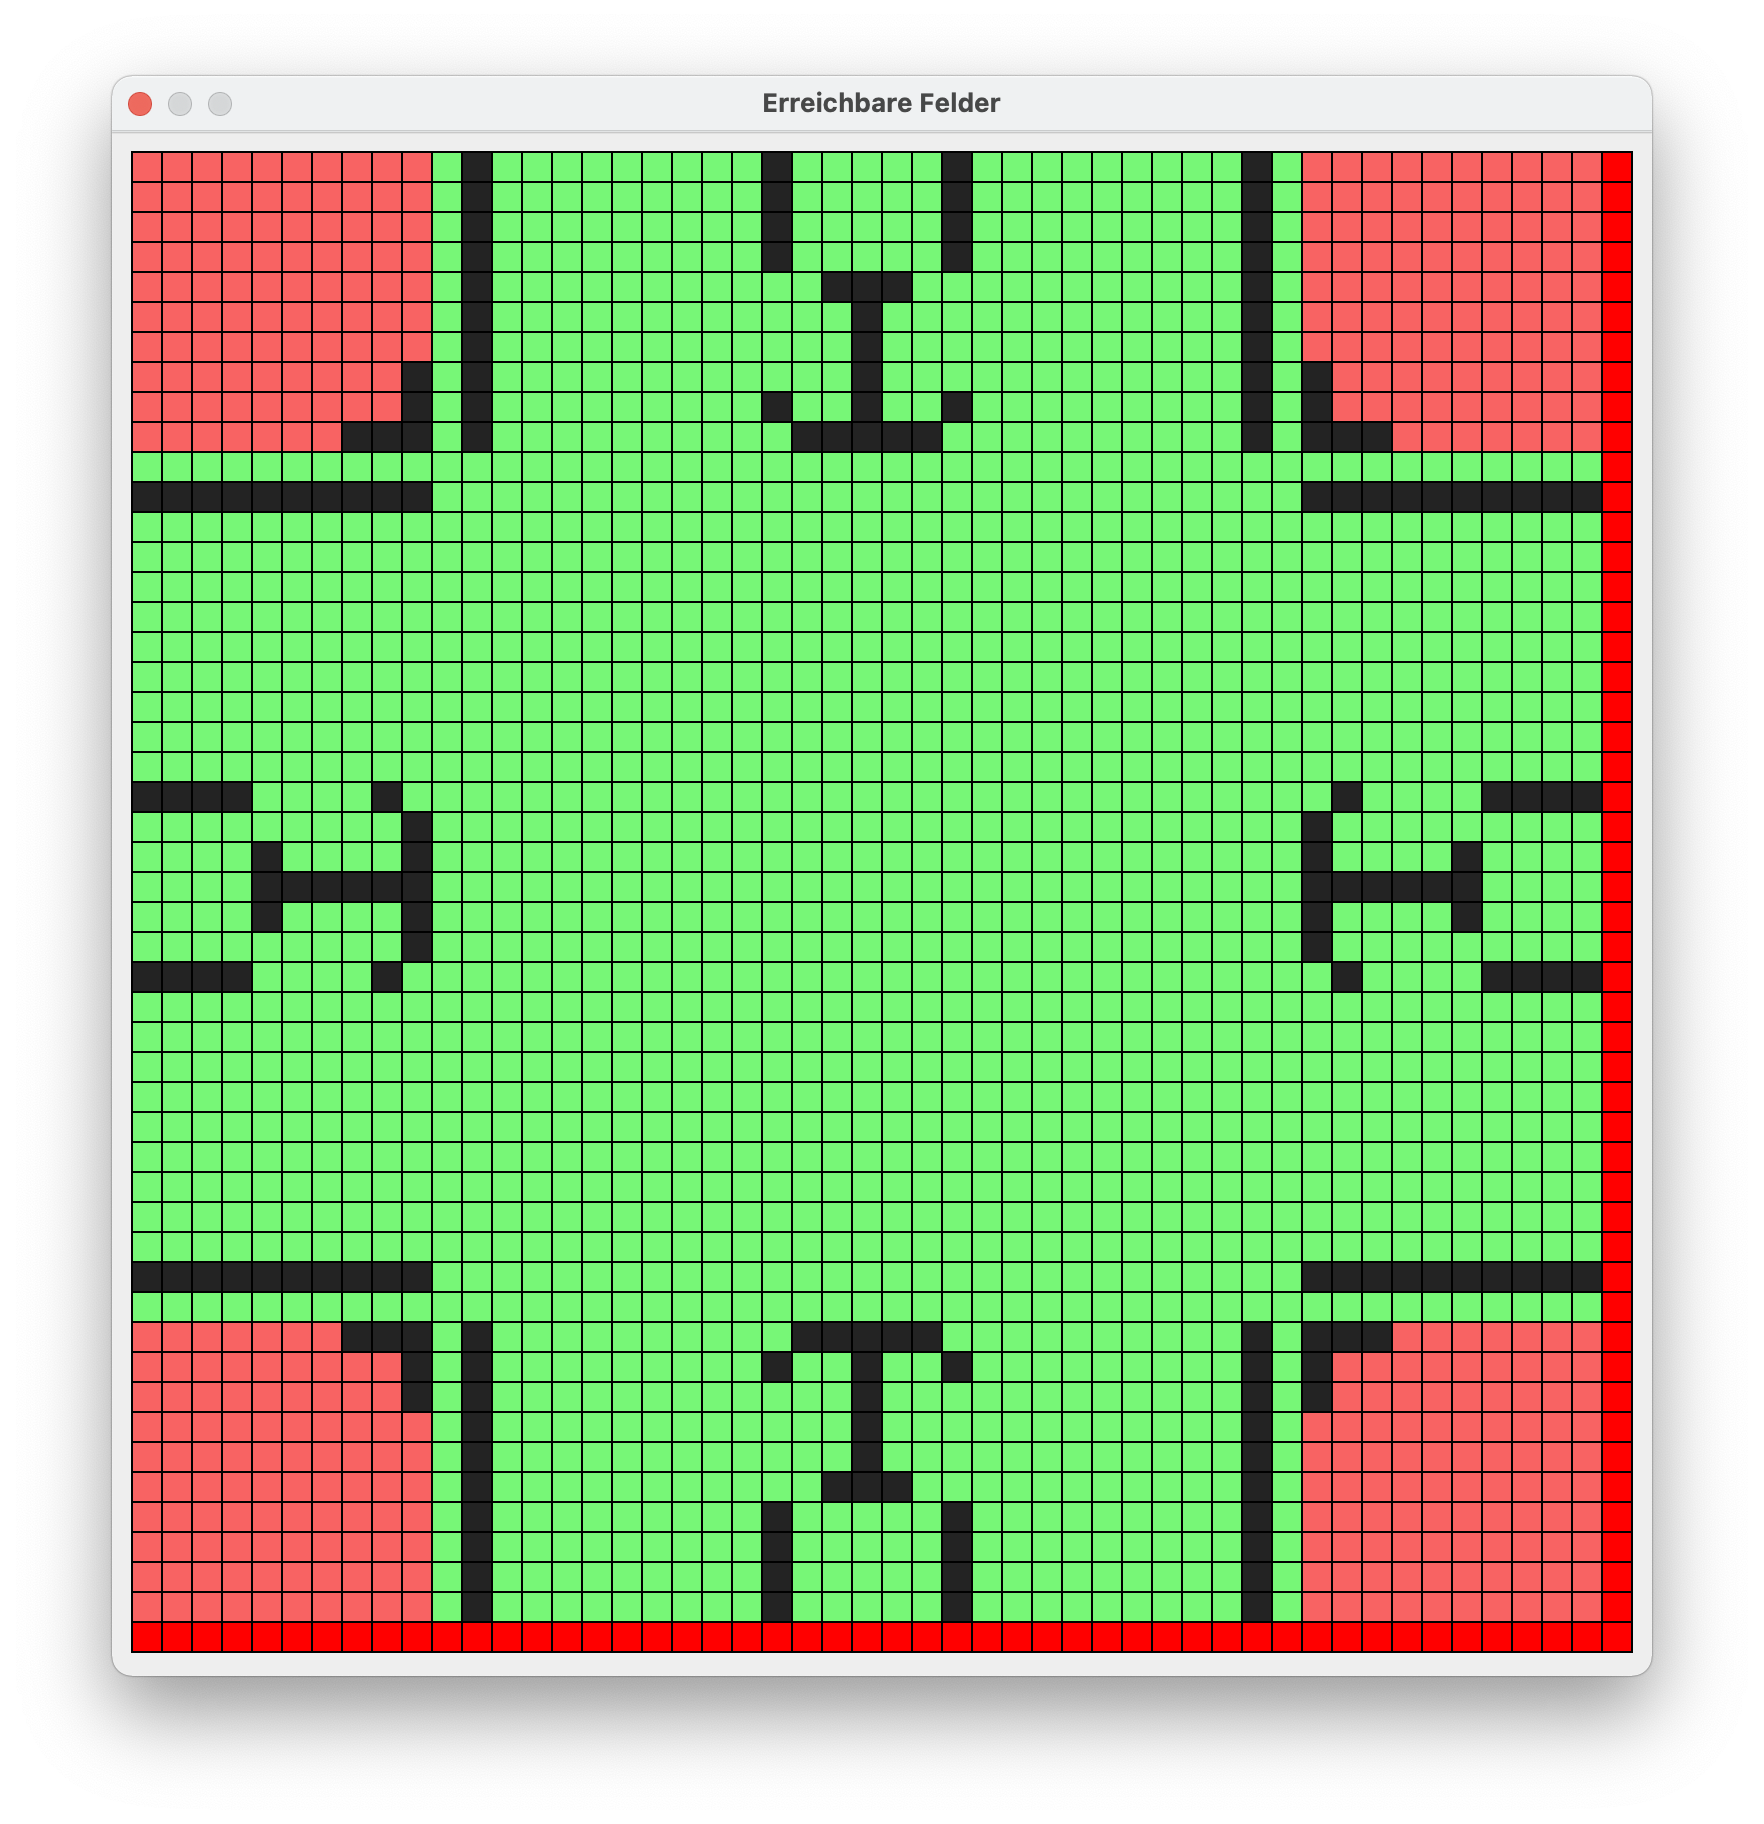
\includegraphics[width=0.48\linewidth]{pics/maps/field2021_01_3p}
    \captionof{figure}[Comp3p]{Dreispielerkarte inkl. erreichbare Felder in Gr\"un (rechts)}
    \label{fig:comp-3p}
\end{minipage}
\vspace{1em}

Diese Dreispielerkarte ist nach dem gleichen Prinzip wie die vorherige Karte aufgebaut.
Jedoch kann man auf dieser Karte 32 zus\"atzliche Bonussteine erreichen.
Die Besonderheit liegt jedoch darin, dass sie jeweils nur aus zwei Richtungen erreichbar sind.
Somit werden diese Felder erst sehr sp\"at im Spielverlauf erobert, wodurch sich das Spiel am Ende drastisch ver\"andern kann.
Der Client verf\"ugt \"uber eine M\"oglichkeit erreichbare Spezialsteine zu finden und bei der Zugauswahl explizit nach diesen zu filtern.

\subsection{Comp2021 - Vierspielerkarte}\label{subsec:comp2021-4p}

\vspace{1em}
\begin{minipage}{\linewidth}
    \centering
    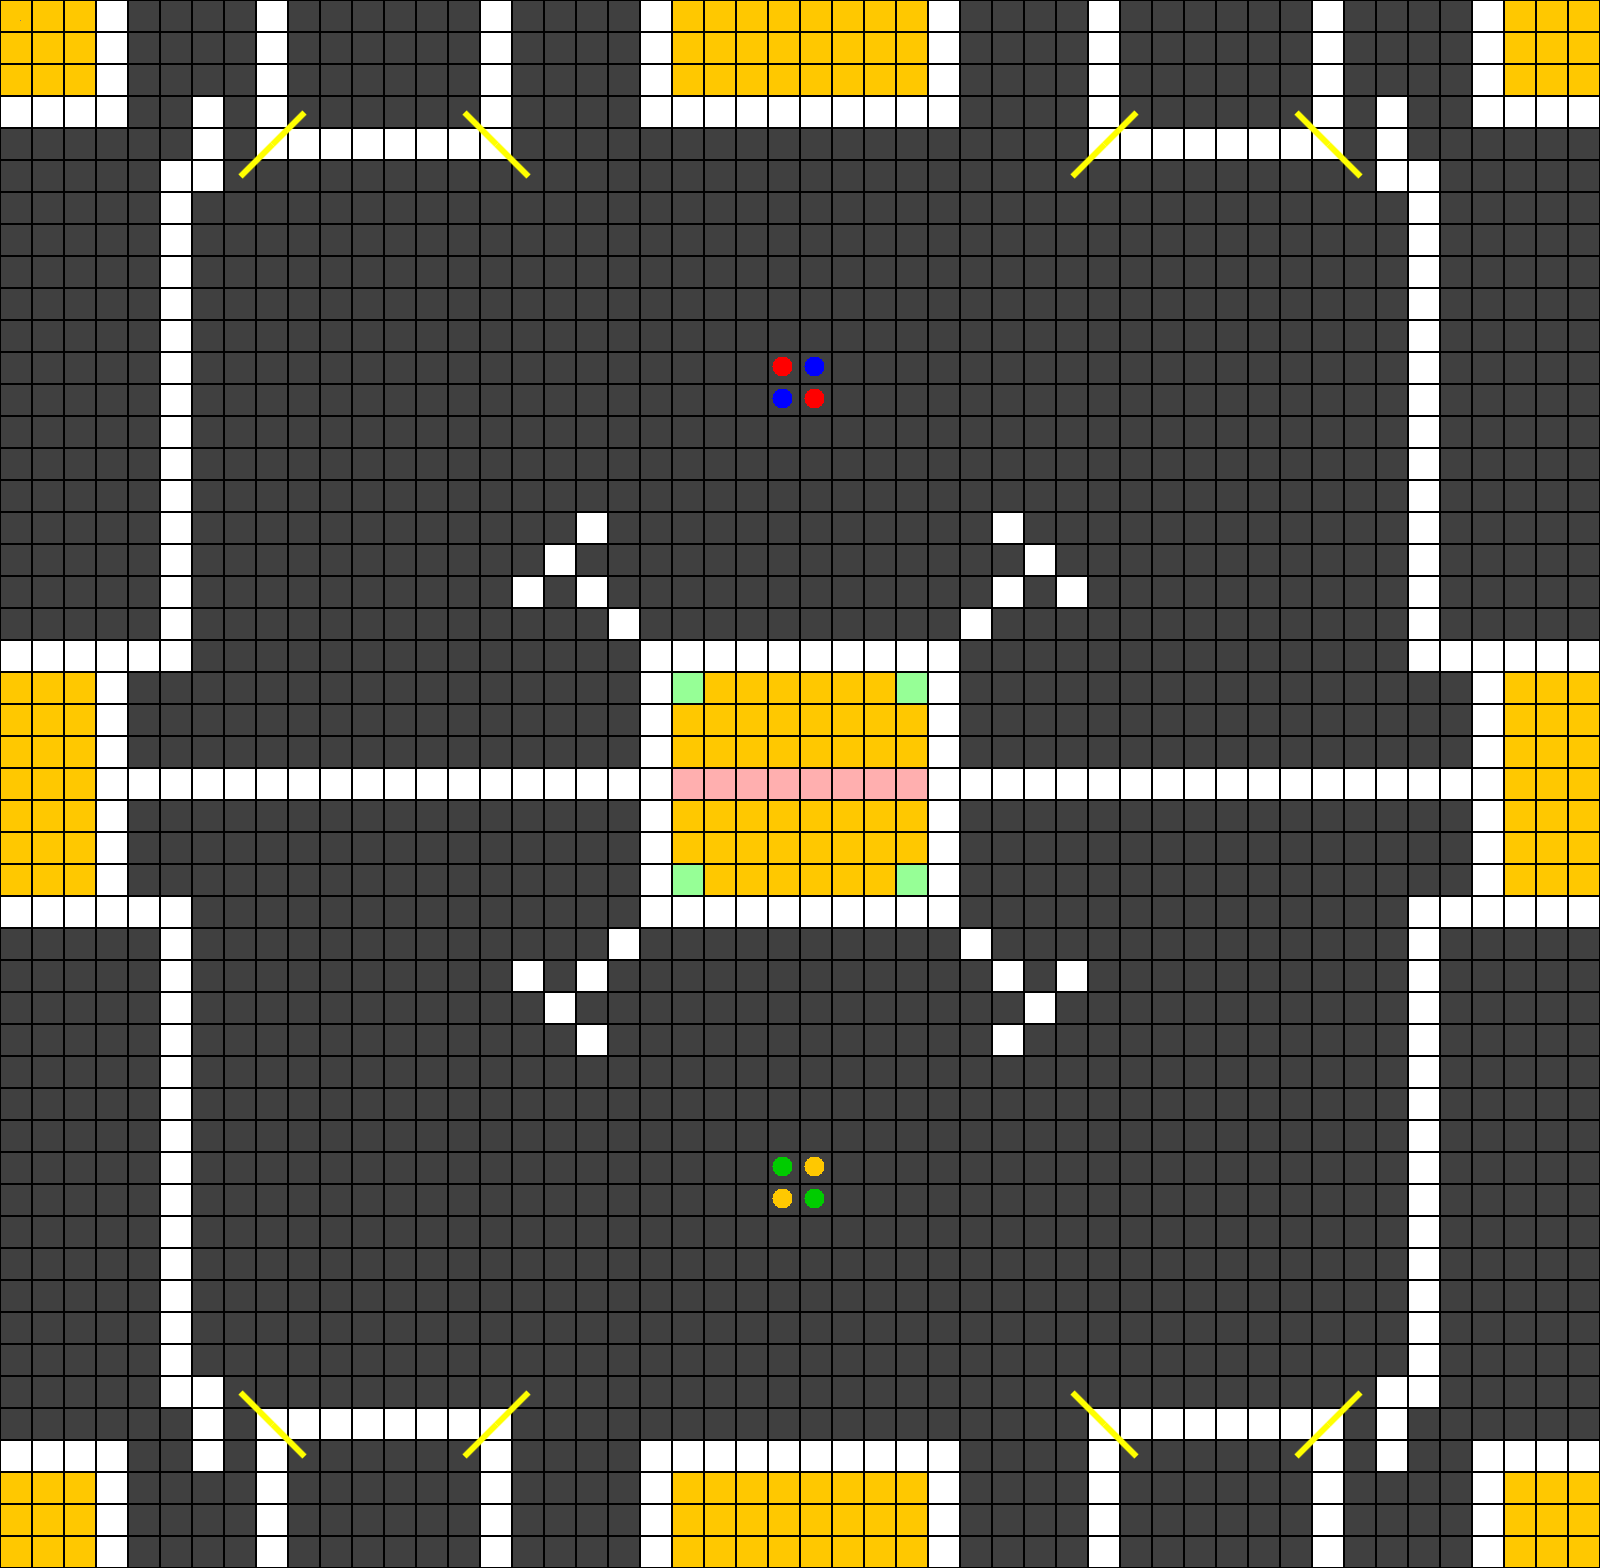
\includegraphics[width=0.49\linewidth]{pics/maps/comp2021_01_4p}
    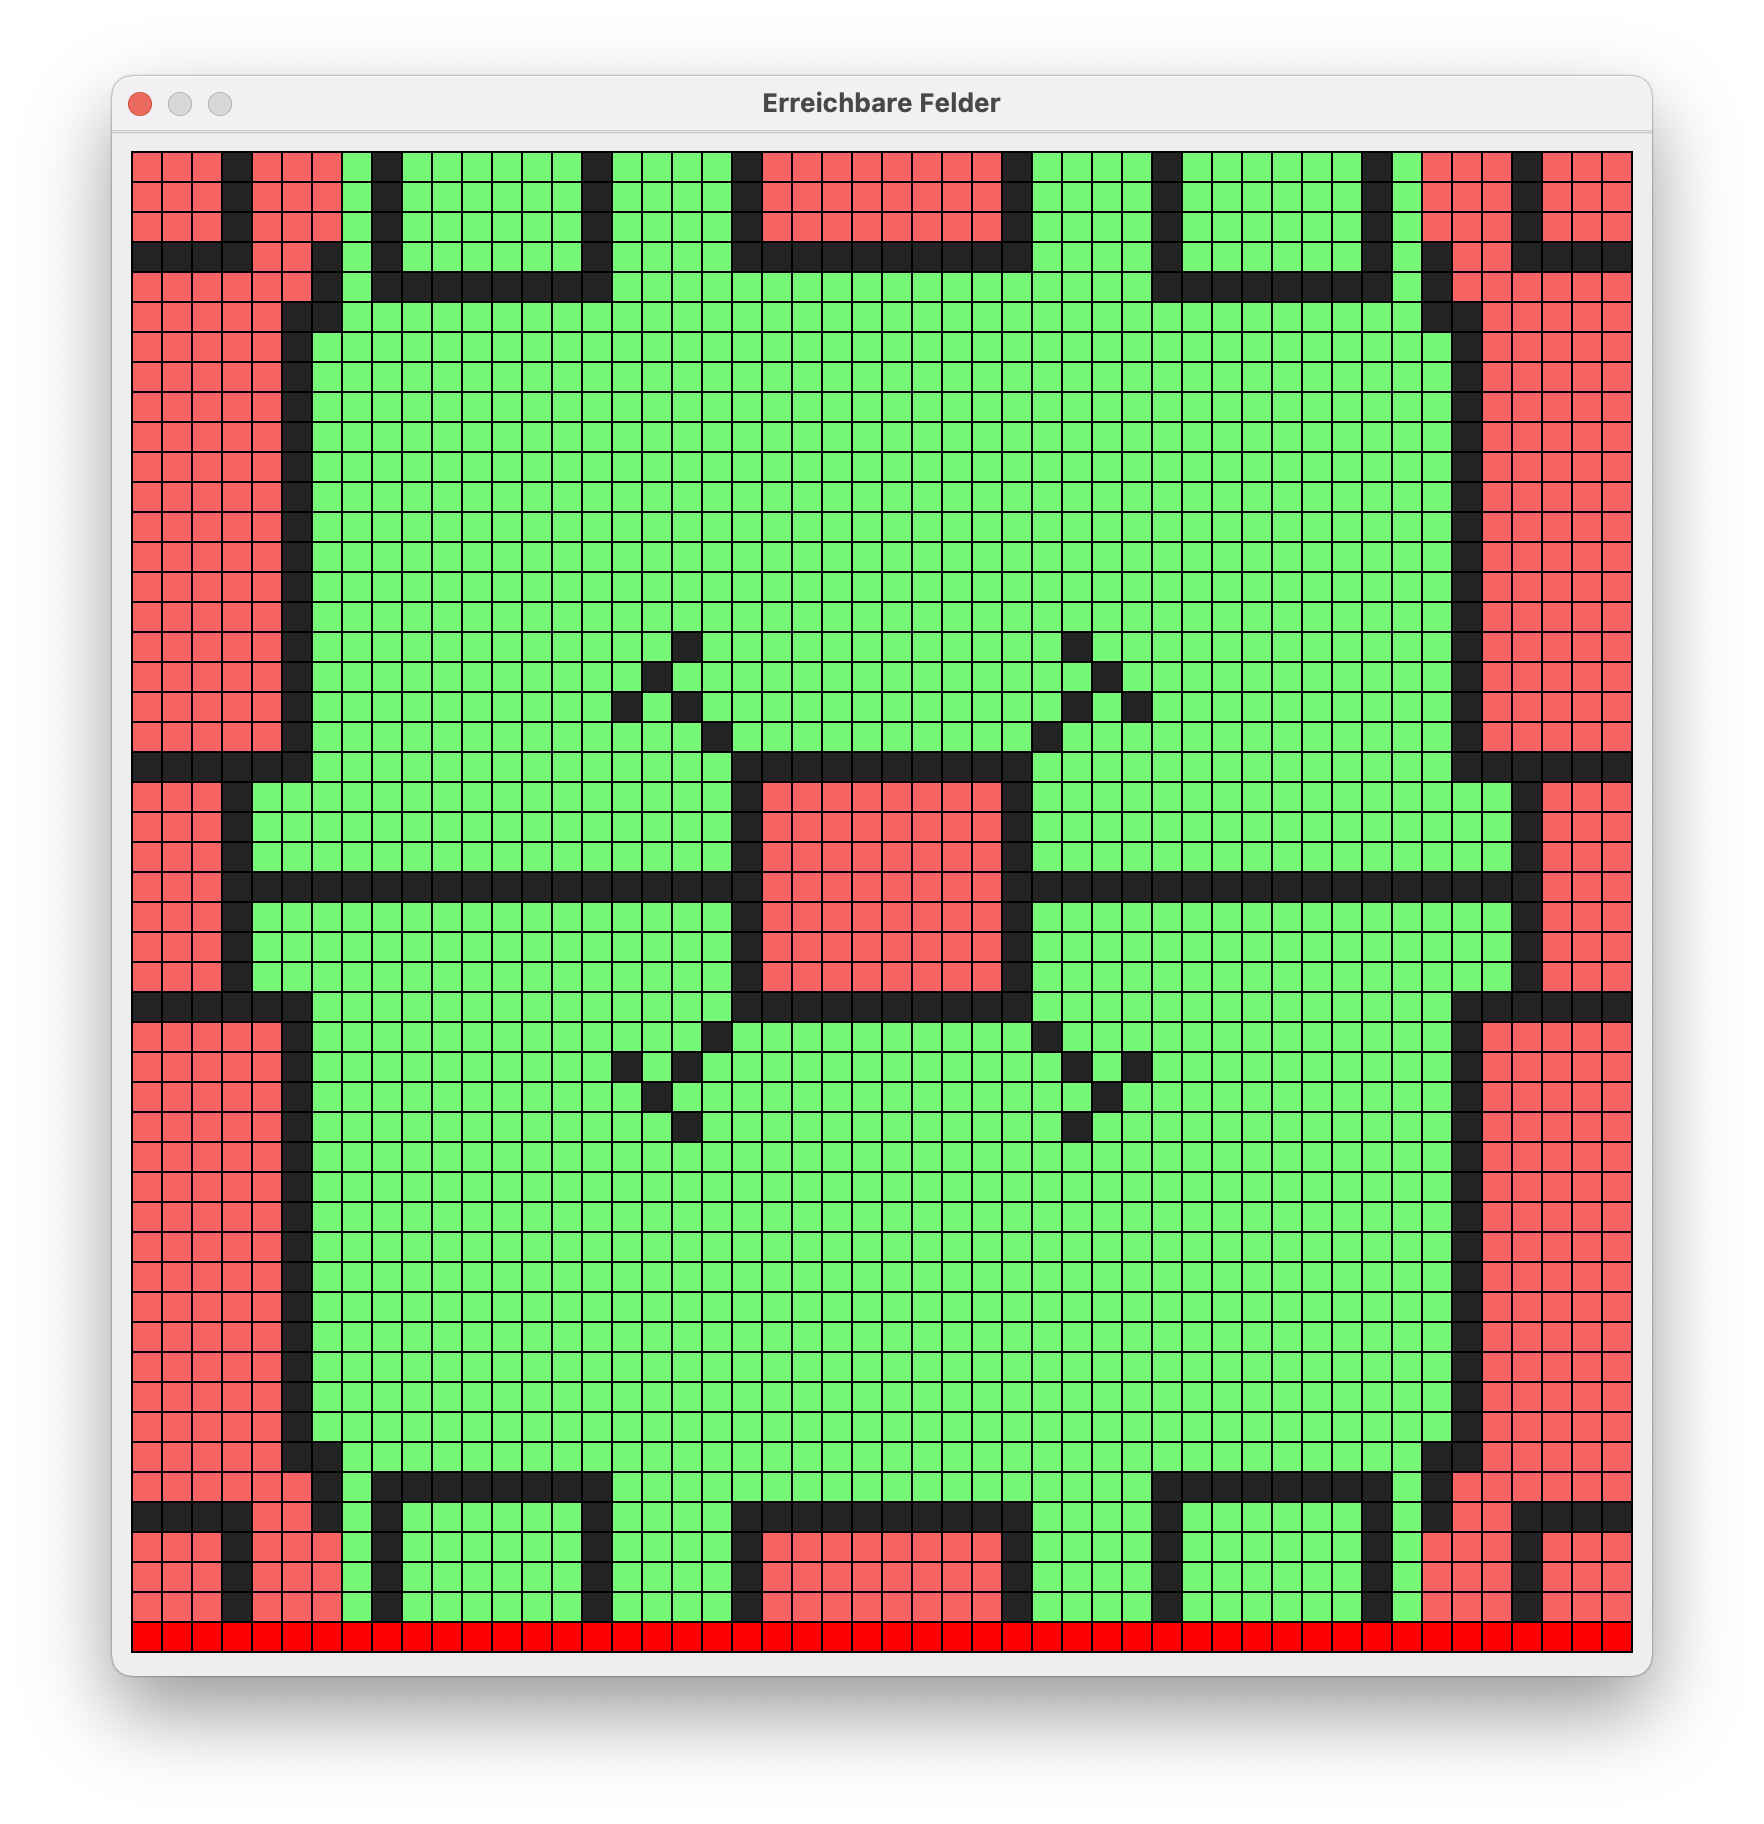
\includegraphics[width=0.48\linewidth]{pics/maps/field2021_01_4p}
    \captionof{figure}[Comp4p]{Vierspielerkarte inkl. erreichbare Felder in Gr\"un (rechts)}
    \label{fig:comp-4p}
\end{minipage}
\vspace{1em}

Auf dieser Karte gibt es eine gro"se Menge von Spezialsteinen, welche jedoch alle nicht erreichbar sind.
Wenn ein Client speziell in die Richtung von Spezialsteinen ziehen m\"ochte, wird dieser damit verwirrt.
Die Besonderheit diese Map liegt zudem darin, dass die linken und rechten Seiten nicht erreichbar sind.
Dies liegt daran, dass man nur aus einer Richtung in diese Bereiche ziehen kann und damit diese Felder nicht einnehmbar sind.
Dadurch wird der prozentuale Spielfortschritt ohne Ber\"ucksichtigung unerreichter Spielfelder stark verf\"alscht.
Dieser Client erkennt somit die prozentuale Belegung wesentlich genauer als andere Clients.
Zudem k\"onnen sich auf dieser Karte die zwei Zweiergruppen nicht gegenseitig beeinflussen, da sie nur in einer H\"alfte spielen.

\subsection{Comp2021 - Achtspielerkarte}\label{subsec:comp2021-8p}

\vspace{1em}
\begin{minipage}{\linewidth}
    \centering
    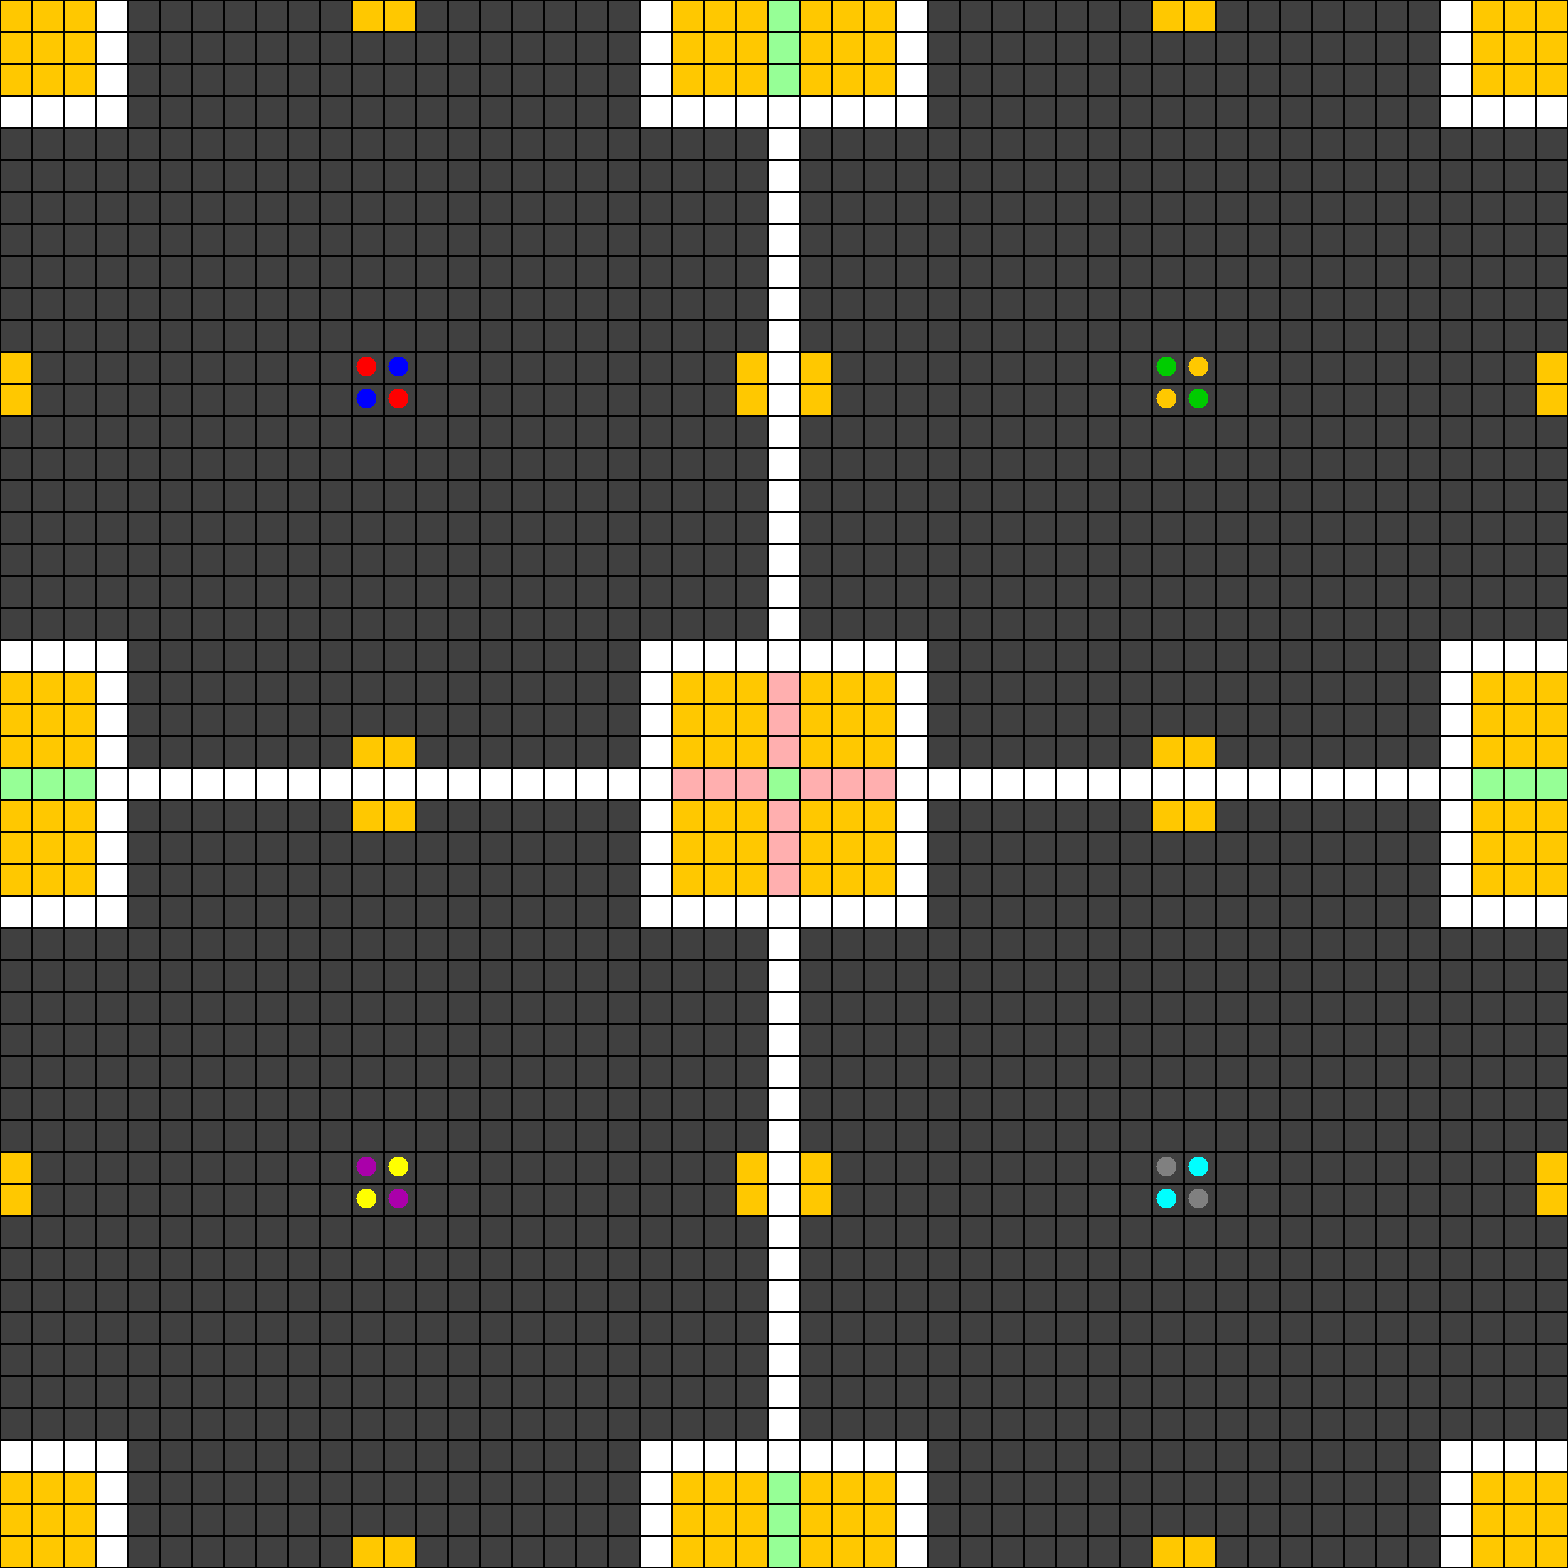
\includegraphics[width=0.49\linewidth]{pics/maps/comp2021_01_8p}
    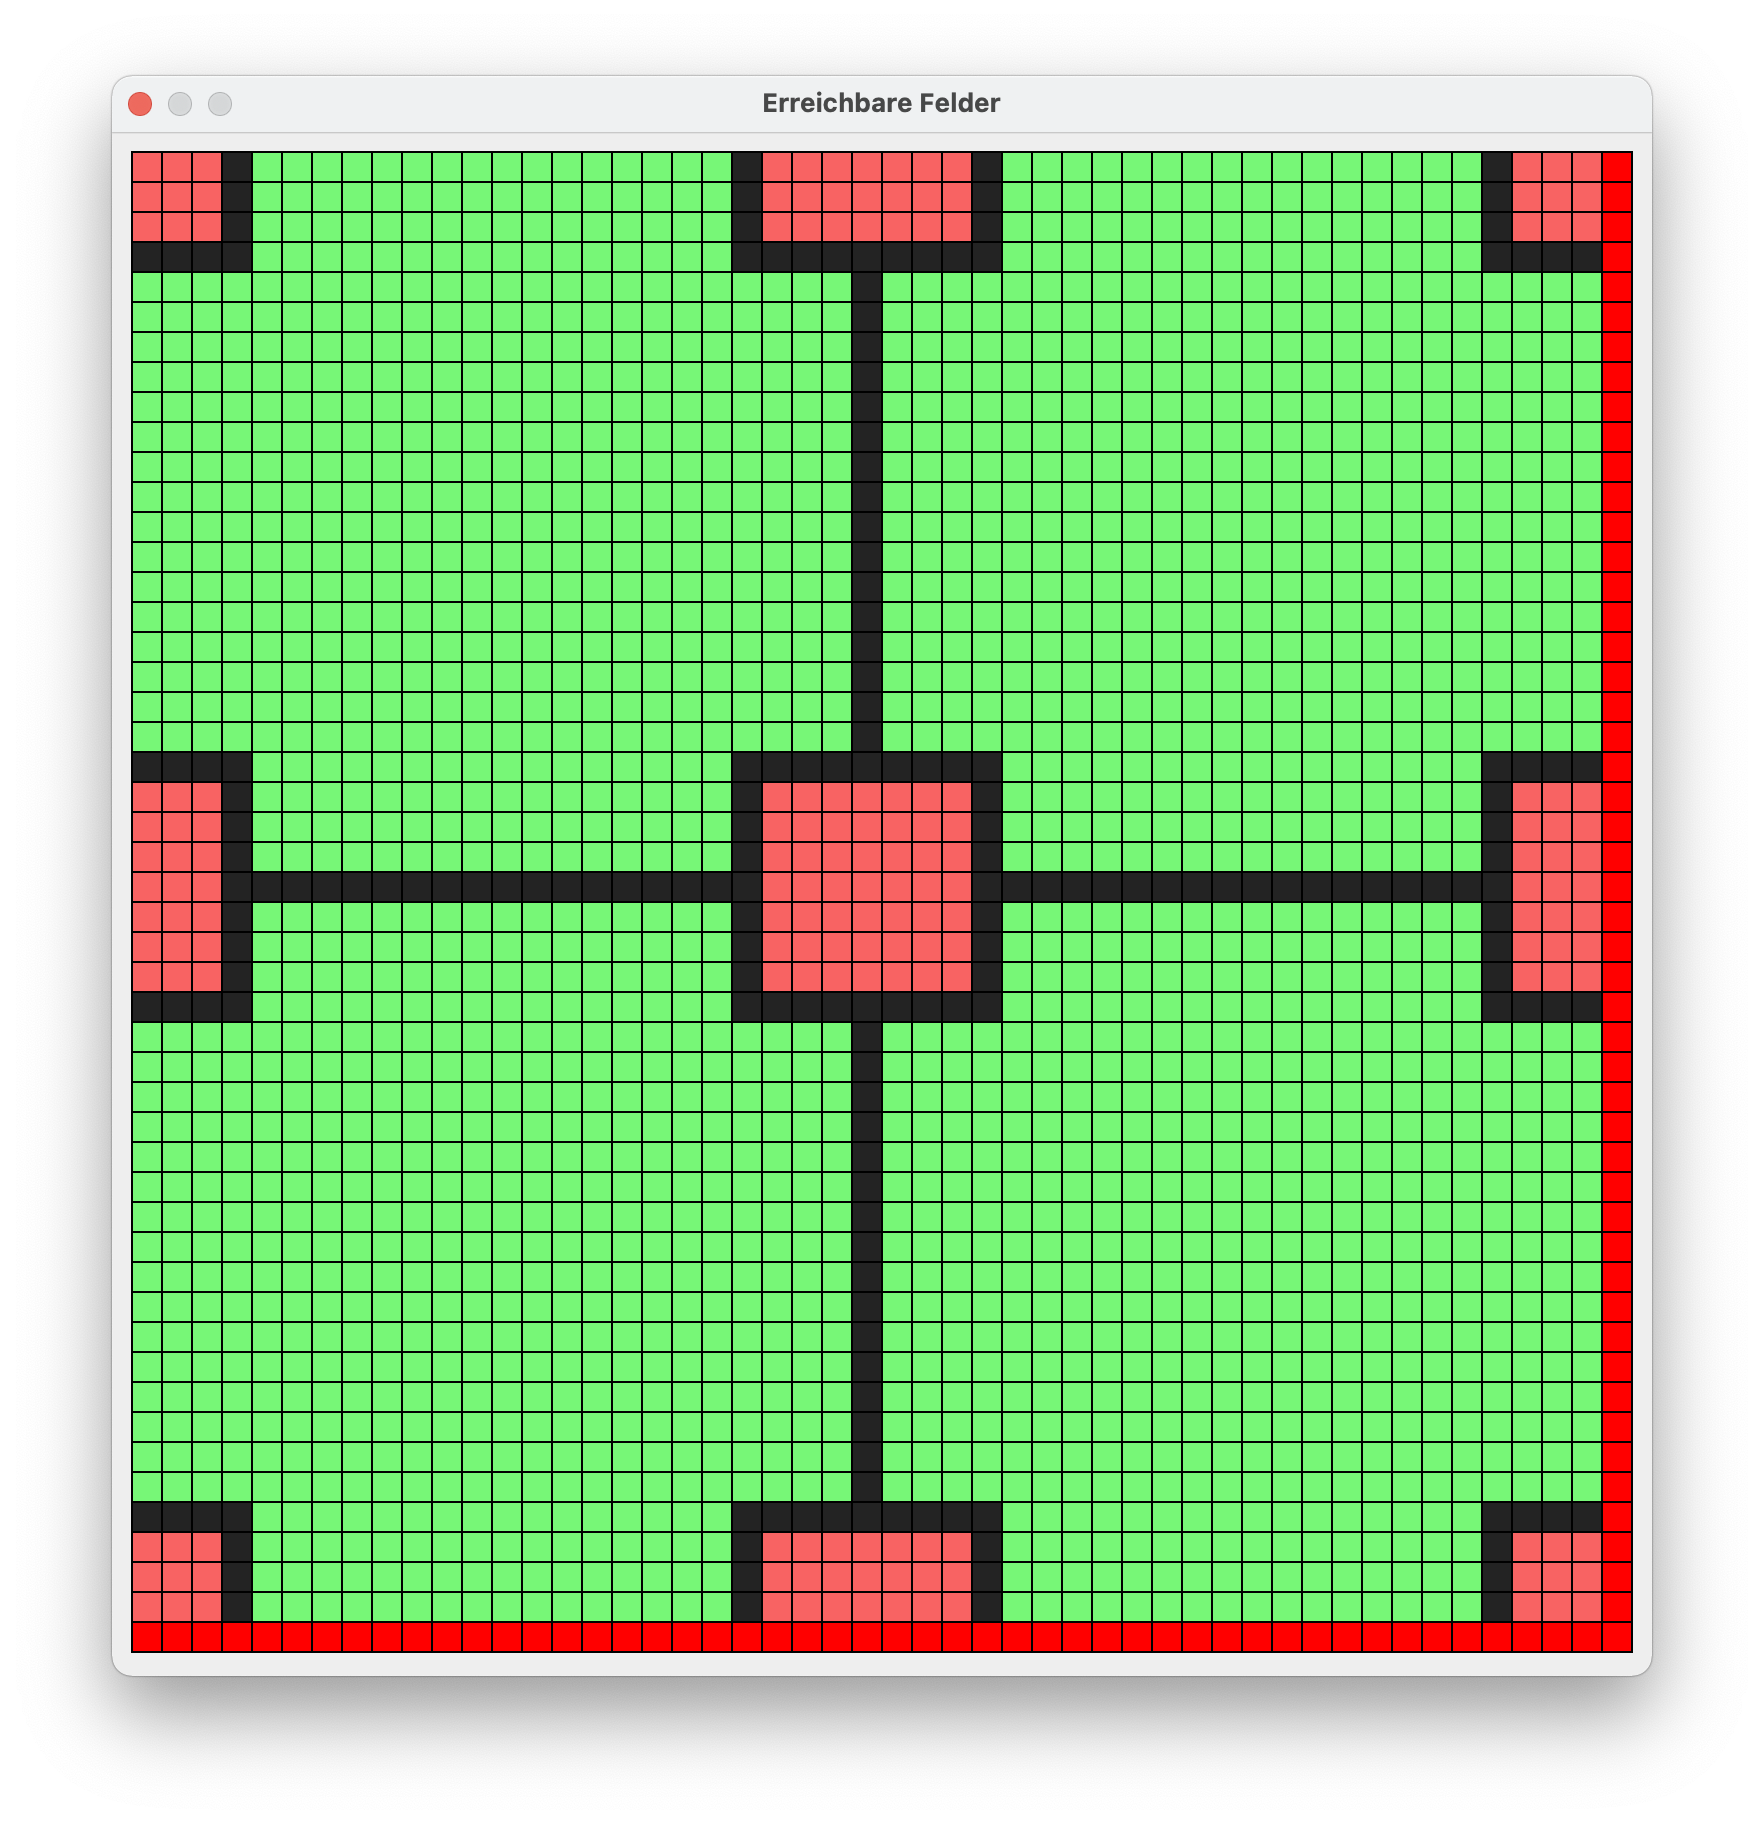
\includegraphics[width=0.48\linewidth]{pics/maps/field2021_01_8p}
    \captionof{figure}[Comp8p]{Achtspielerkarte inkl. erreichbare Felder in Gr\"un (rechts)}
    \label{fig:comp-8p}
\end{minipage}
\vspace{1em}

Die Achtspielerkarte ist \"ahnlich wie die vorherige Karte aufgebaut.
Es ist nur ein Bruchteil der Spezialsteine erreichbar.
Zudem spielen hier vier Zweiergruppen unabh\"angig gegeneinander.
Die Heuristik dieses Clients verf\"ugt \"uber die M\"oglichkeit, Spieler die einen selbst nicht erreichen k\"onnen zu \"uberspringen.
Dabei wird ein g\"ultiger und guter Zug ausgew\"ahlt und \"ahnlich wie bei BFS+ mit diesem Zug im Suchbaum weitergearbeitet.
Dadurch wird der Suchbaum nicht unn\"otig aufgeb\"aht, wodurch in gro"sere Tiefen gesucht werden kann.
Mithilfe dieser Reduktion des Suchbaumes werden unn\"otige Berechnungen vermieden und somit auch bei Achtspielerkarten eine Suchbaumtiefe von 10 und gr\"o"ser erm\"oglicht.

\bigskip
\newpage